\chapter{Active Syntax of Recipient Ditransitives}\label{ch:active}
\section{Introduction}
This chapter focuses on the proper analysis of active recipient ditransitives. Using data from Germanic languages, I support the claim that all recipients are base generated as dative PPs in the specifier of an applicative phrase. One of the main goals of this chapter is to distinguish this analysis of recipients from the proper analysis of goals, which are often confused with recipients (due to a large degree of semantic overlap). Goals are the end point of a path of motion. Recipients, on the other hand, are the new possessors after a transfer of possession event (in which no movement is necessary), as described in the previous chapter. Given that moving something from one persons domain to another is a standard way of enacting a transfer of possession, these two notions can often be introduced by the same verbs, which can lead to syntactic ambiguity. The determination of whether the argument of one of these verbs is more similar to the recipient or goal proto-role is determined by each speech community.

The main empirical puzzle that this chapter addresses is the relationship between the three forms found with certain High German verbs of motion (\ref{ex:german-forms}) and the two forms of English dative shift (\ref{ex:dat-shift}). These patterns are replicated across the other Germanic languages, and relevant data from other languages are also examined. With verbs like High German, \textit{schicken} ``to send'', a goal/recipient can occur in three different positions: (\ref{ex:german-1}) marked with dative before an accusative marked theme, (\ref{ex:german-2}) marked with dative after an accusative marked theme, and (\ref{ex:german-3}) introduced by the preposition \textit{an} ``to/on'' after an accusative marked theme. In Modern American English, the same argument can occur in the following positions: (\ref{ex:english-1}) unmarked before an unmarked theme or (\ref{ex:english-2}) introduced by the preposition \textit{to} after an unmarked theme. I will argue that English (\ref{ex:english-1}) is always a reflection of German (\ref{ex:german-1}) and the English (\ref{ex:english-2}) is ambiguous between German (\ref{ex:german-2}) and (\ref{ex:german-3}) with the syntactic ambiguity reflecting a semantic difference between a recipient and goal interpretation.

\begin{exe}
	\ex High German, Dative--Preposition Alternation: \label{ex:german-forms}
	\begin{xlist}
		\ex \label{ex:german-1} \gll Ich habe der Frau das Buch geschickt\\
			I.NOM have the.DAT woman the.ACC book sent\\
			 \trans `I sent the woman the book.'
		 \ex \label{ex:german-2} \gll Ich habe das Buch der Frau geschickt\\
			 I.NOM have the.ACC book the.DAT woman sent\\
			 \trans `I sent the woman the book.'
		 \ex \label{ex:german-3} \gll Ich habe das Buch an die Frau geschickt\\
			 I.NOM have the.ACC book to the.ACC woman sent\\
			 \trans `I sent the book to the woman.'
	\end{xlist}
	\exr{ex:dat-shift} English, Dative Shift:
	\begin{xlist}
		\exr{ex:english-1} I sent the woman the book.
		\exr{ex:english-2} I sent the book to the woman.
	\end{xlist}
\end{exe}

German and Icelandic encode the distinction between the goals and recipients with the morphological distinction between prepositions and dative case. This morphological distinction is coupled with a syntactic distinction in base generation position. Using data from other Germanic languages, I argue that the distinction between prepositions and dative case morphology does not always clearly align with this semantic difference and thus that the presence/absence of a preposition cannot be used as a diagnostic for syntactic structure. The dative PP analysis described in the previous chapter is used to account for these mismatches. The presence/absence of \textit{to} in dative shift can then be accounted for using contextual allomorphy (i.e. the same mechanism that determines that the plural of \textit{cat} is \textit{cats}, but that the plural of \textit{sheep} is \textit{sheep}). Evidence from Swedish and the history of English is brought to support this KP + contextual allomorphy account.

After demonstrating that recipients and goals are different constructions, I argue that theme--recipient word orders (e.g. ``I gave the theme to the recipient'') are derived via VP-internal scrambling. I present typological evidence suggesting that the recipient--theme order is base generated and then give data from High German that suggests that the mechanism for deriving the theme--recipient order is scrambling. I finish by presenting evidence from Low German that demonstrates that complex surface morphology is unnecessary for scrambling to occur. Finally, I conclude by reviewing the argument for the conclusions introduced above.

\section{Goals and Recipients}
	\subsection{Introduction}
	This section focuses on arguing that goals and recipients are distinct thematic roles and therefore introduced in distinct constructions in natural language. As discussed in the previous chapter, my claims are specifically about the syntactic structures associated with recipients. The comparison with goals provides an example of how concepts that are closely related semantically can have quite different syntactic realisations. It is necessary to emphasise this point, because this distinction is poorly marked in English and this has confused research about the structure of English ditransitives (see \citet{Hovav.2008} for a full discussion). I show how evidence from Icelandic and German (both of which maintain synthetic dative case forms) support different thematic roles and base generation positions for recipients and goals. I then review evidence from modern English that shows that this difference also applies in English with the caveat that some surface forms are ambiguous between a recipient and goal interpretation. 

	In Icelandic, recipients are typically marked with dative case marking. Indeed, \cite{Thrainsson.2007}, in his grammar of Icelandic, describes the availability of PP-alternants as follows: 
	\begin{quotation}
	\ldots in Icelandic the PP-alternative is pretty much restricted to verbs of sending (i.e., where the IO is an actual goal of some sort of movement) \ldots Interestingly, if the verbs \textit{gefa} `give' and \textit{selja} `sell' can be interpreted as having a directional sense, then it becomes normal to use the prepositional variant in Icelandic:
	\begin{exe}
		\ex Icelandic: \label{ex:icelandic-goals}
		\begin{xlist}
		\ex \gll \'{E}g gaf b\ae kurnar til H\'ask\'olab\'okasafnsins\\
		I.NOM gave books.the.ACC to University.Library.the.GEN\\
		\trans `I gave the books to the University Library'
		\ex \gll \th eir seldu skipi\dh til Englands\\
		they.NOM sold ship.the.ACC to England.GEN\\
		\trans `They sold the ship to England.'
		\end{xlist}
	\end{exe}
	In the last example a dative IO would not be a possibility since `England' would not be the actual recipient (unless one was talking about the English (or British) state or some such \ldots \citep[fn 64]{Thrainsson.2007}
	\end{quotation}
	For German, the same pattern holds, prepositional objects with \textit{an} ``to (for animate goals)'' or \textit{nach} ``to (for inanimate goals)'' are restricted to verbs of motion (i.e. they cannot occur with pure verbs of transfer, e.g. \textit{geben} `give'). Also, when dative case is used with verbs of motion, an obligatory recipient interpretation is derived, i.e. the theme must actually have been transferred into the possession of the recipient. In the following examples (\ref{ex:german-goals}), the verb \textit{schicken} ``send'' can take both dative and prepositional objects. When a dative object is used, then the dative must actually gain possession of the theme. With a prepositional complement, change of possession need not occur. This difference supports the idea that the dative encodes recipients (the end point of a transfer of possession), while the prepositional varieties encode goals (end point of a movement path, which can be interrupted).

\begin{exe}
	\ex High German:\label{ex:german-goals}
	\begin{xlist}
		\ex[\#]{\gll Er hat \textbf{Maria} einen Brief geschickt, aber er ist bei ihr nicht angekommen\\
		he.NOM has \textbf{Maria} a.ACC letter sent, but he.NOM is by her.DAT not arrived\\
\trans `He sent Maria a letter, but it has not reached her.'}
\ex[\#]{\gll Er hat einen Brief \textbf{Maria} geschickt, aber er ist bei ihr nicht angekommen\\
		he.NOM has a.ACC letter \textbf{Maria} sent, but he.NOM is by her.DAT not arrived\\
\trans `He sent a letter to Maria, but it has not reached her.'}
\ex[ ]{\gll Er hat einen Brief \textbf{an} \textbf{Maria}  geschickt, aber er ist bei ihr nicht angekommen\\
he.NOM has a.ACC letter \textbf{to} \textbf{Maria} sent, but he.NOM is by her.DAT not arrived\\
\trans `He sent a letter to Maria, but it has not reached her.'}
	\end{xlist}
\end{exe}

	German also provides evidence that the dative recipients and prepositional goals are syntactically distinct. While German has fairly free word order, topicalised VPs provide a window into which word orders are possible within the verb phrase. With dative recipients, both recipient--theme and theme--recipient word orders are possible in topicalised VPs.

	\begin{exe}
		\ex\label{ex:german-VP-top} High German, VP-topicalisation:
		\begin{xlist}
			\ex \gll  Dem Mann das Buch gegeben habe ich, (nicht der Frau dEN Film geschenkt).\\
			the.DAT man the.ACC book given have I, (not the.DAT woman the.ACC film sent).\\
			\trans `It was giving the man the book that I did (not sending the woman the film).'
			\ex \gll Das Buch dem Mann gegeben habe ich, (nicht dEN Film der Frau geschenkt).\\
			the.ACC book the.DAT man given have I, (not the.ACC film the.DAT woman sent).\\
			\trans `It was giving the book to the man that I did (not sending the film to the woman).\\
		\end{xlist}
	\end{exe}

	However, with prepositional goals, only the theme--goal order is possible, suggesting that prepositional goals start below the theme in a prepositional object construction and are unable to move above the theme inside the VP. Here, the main point is that the prepositional goals and dative recipients do not show the same syntactic pattern indicating that they occupy distinct syntactic positions. A full analysis of these differences is provided in Section \ref{sec:synrecp}. The basic outline is that recipients are introduced in the specifier of an applicative phrase (i.e., in a higher functional projection above the main verb), while goals are introduced as the complement of the main verb. 

	\begin{exe}
		\ex\label{ex:hg-vp-top-goals} High German, VP-topicalisation:
		\begin{xlist}
			\ex[*]{ \gll  An den Mann das Buch geschickt habe ich, (nicht an die Frau dEN Film übergeben).\\
			to the.ACC man the.ACC book sent have I, (not to the.ACC woman the.ACC film delivered).\\
		\trans `It was sending to the man the book that I did (not delivering to the woman the film).'}
		\ex[ ]{\gll Das Buch an den Mann gegeben habe ich, (nicht dEN Film an die Frau übergeben).\\
			the.ACC book to the.ACC man given have I, (not the.ACC film to the.ACC woman delivered).\\
		\trans `It was sending the book to the man that I did (not delivering the film to the woman).\\}
		\end{xlist}
	\end{exe}

	\subsection{Two \textit{to}s in English}
	Much confusion has occurred in the discussion English ditransitives from combining recipient and non-recipient ditransitives in the same analysis. As discussed above, there is good cross-linguistic evidence that non-recipient ditranstives have a different structure than recipient ditransitives (and are therefore not probative of recipient constructions). \cite{Levinson.2005} and \cite{Hovav.2008} show that there are (at least) two \textit{to}s in English: one that introduces recipients and one that introduces goals. Any argument that uses verbs of motion (e.g. \textit{send}) is going to run afoul of this ambiguity.

	One of the best arguments for the distinction between recipient and goal \textit{to} comes from wh-questions. Goals introduce a location and can therefore be questioned with \textit{where}, while recipients are not locative and therefore do not allow for \textit{where}-questions.

	\begin{exe}
		\ex English, Recipients:\label{ex:eng-rec-wh}
		\begin{xlist}
			\ex[ ]{Who did you give the package to?}
			\ex[*]{Where did you give the package to?}
		\end{xlist}
		\ex English, Goals:\label{ex:eng-goal-wh}
		\begin{xlist}
			\ex[ ]{Who did you send the package to?}
			\ex[ ]{Where did you send the package to?}
		\end{xlist}
	\end{exe}

	\cite{Hallman.2015} provides additional evidence supporting a distinction between goal and recipient interpretations (or at least between \textit{to} marked recipients and prepositional object constructions). He notes that \textit{to}-marked recipients pattern with bare recipients and not with prepositional objects in their ability to control into purpose clauses. In both the recipient--theme and theme--recipient orders (\ref{ex:hallman-rec}), the recipient is able to bind PRO in the purpose clause and the theme is able to bind the empty category object. Crucially, this means that the recipient needs to be higher than $\bar{V}$, which is the site of purpose clause attachment.
\begin{exe}
	\ex English \citep[exx 6 \& 7]{Hallman.2015}:\label{ex:hallman-rec}
\begin{xlist}
\ex Mary gave John$_{i}$ a puppy$_{k}$ [PRO$_{i}$ to play with e$_{k}$].
\ex Mary gave a puppy$_{k}$ to John$_{i}$ [PRO$_{i}$ to play with e$_{k}$].
\ex Mary sent John$_{i}$ a manuscript$_{k}$ [PRO$_{i}$ to read e$_{k}$]
\ex Mary sent a manuscript$_{k}$ to John$_{i}$ [PRO$_{i}$ to read e$_{k}$]
\end{xlist}
\end{exe}%12 - Recipient--theme and theme--recipient purpose clauses

This is crucially different from the behaviour of prepositional objects in prepositional object constructions (e.g. as introduced by `put'). The prepositional objects scope under the purpose clause and cannot control into it (\ref{ex:hallman-poc}). Example \ref{ex:hallman-control-2} shows that the ungrammaticality comes from the presence of the purpose clauses, as opposed to some inherent problem in the matrix POC constructions.

\begin{exe}
	\ex English \citep[ex 9]{Hallman.2015}:\label{ex:hallman-poc}
	\begin{xlist}
		\ex[*]{Mary put the child$_{k}$ on the horse$_{i}$ [PRO$_{i}$ to carry e$_{k}$]}
		\ex[*]{Mary led the horse$_{k}$ to John$_{i}$ [PRO$_{i}$ to feed e$_{k}$]}
		\ex[*]{Mary immersed the cloth$_{k}$ in oil$_{i}$ [PRO$_{i}$ to permeate e$_{k}$]}
		\ex[*]{Mary placed the planting pots$_{k}$ under the tomato vines$_{i}$ [PRO$_{i}$ to grow over e$_{k}$]}
	\end{xlist}
	\ex \label{ex:hallman-control-2}English \citep[ex 10]{Hallman.2015}:
	\begin{xlist}
		\ex[ ]{Mary put the child on the horse}
		\ex[ ]{Mary led the horse to John}
		\ex[ ]{Mary immersed the cloth in oil}
		\ex[ ]{Mary placed the planting pots under the tomato vines}
	\end{xlist}
\end{exe}

Hallman argues that this control asymmetry can be captured by having the recipient \textit{to} and goal \textit{to} in different syntactic positions. Assuming that purpose clauses are adjoined to the edge of V-bar, recipient \textit{to} must occur outside of VP in order to be able to bind into the purpose clause. In the previous chapter, I showed how the main difference between the applicative analysis of recipients and the other currently viable analyses was that the applicative analysis put the recipient in a higher functional projection than the VP (and thus positions the recipient to be able to bind into VP level material). All the other analyses had the recipient as either the complement of the main verb or part of the complement of the main verb and thus underneath the purpose clause and unable to bind into it. The goal \textit{to} as part of a prepositional object construction is placed inside the VP and thus is unable to bind into the purpose clause. The exact structures under consideration are discussed in the end of this chapter; here the essential point is that even in English there is good evidence for a syntactic difference between recipients and goals.

\section{Morphology and Dative Marking}
	\subsection{Typology of Morphosyntactic Marking}
	I argued above that goals and recipients have distinct syntactic positions. Also, in High German and Icelandic, recipients were marked with dative case while goals were introduced by prepositions. The goal of this section is to argue that the preposition/case distinction is a surface morphological property and that both goals and recipients are introduced as the same type of syntactic object. As discussed in the previous chapter, I argue for an analysis of recipients as being dative PPs.

	One example of the interchangability of case and prepositions in recipient ditransitives comes from certain dialects of High German (in particular the dialects spoken in Alsace, Baden-Württemberg, Switzerland, and Bavaria). In these dialects, the preposition \textit{in} `in/into' or the preposition \textit{an} `on/onto' has come to be used with full noun phrases in cases where standard German has dative case. This occurs even though synthetic dative case is still marked in these dialects \citep{Seiler.2001,Seiler.2003}. If the distinction between case and preposition was deeply syntactic (especially if it correlated with the difference between goals and recipients), syntactic and semantic restrictions on the distribution of prepositional elements is predicted. 
	
	However, \cite{Seiler.2001} claims, using data both from dialect corpora and traditional fieldwork, that ``PDM [Prepositional Dative Marking] is not sensitive to different semantic roles, and PDM does not encode different information than does a bare dative NP.'' He also states that ``the relative order of direct and indirect object in the middle field doesn't cause any asymmetry in the acceptance of PDM.'' Thus, prepositional marking can freely occur with ditransitives in both recipient--theme and theme--recipient orders as seen below \citep{Seiler.2001,Seiler.2003}:
	\begin{exe}
		\ex Zürich German:\label{ex:zurich}
		\gll si schänkt äine \textbf{a} \textbf{de} \textbf{Tristane}\\
		they.NOM sent one.ACC to the Tristan\\
		\trans `The sent one to Tristan \citep[pg. 175]{Seiler.2003}.'
		\ex Luzern German:\label{ex:luzern}
		\gll miir verchauggid \textbf{i} \textbf{de} \textbf{Chunde} nur Mère-Josephine-Poulets\\
		we.NOM sold to the clients only Mere-Josephine chicken\\
		`We sold the clients only Mere-Josephine chicken \citep[pg. 175]{Seiler.2003}.'

	\end{exe}
	Dutch also shows a pattern where prepositional marking is not restricted to certain syntactic positions or thematic roles. In modern Standard Dutch, the prepositions \textit{aan} `to' can be used both with goals and with recipients. When introducing recipients, it must occur in the theme--recipient order, but is also freely available in recipient--theme orders.
	\begin{exe}
		\ex Dutch:\label{ex:dutch-rec-marking}
		\begin{xlist}
			\ex \gll Ik heb een boek *(aan) Jan gegeven\\
			I have a book to John given\\
			\trans `I gave a book to John \citep{Tiersma.1985}.'
			\ex \gll Ik heb (aan) Jan een boek gegeven\\
			I have to John a book given\\
			\trans `I gave John a book \citep{Tiersma.1985}.'
		\end{xlist}
	\end{exe}
	Another example comes from certain dialects of British English. In the previous examples, prepositions occurred in positions that are restricted to synthetic dative case in German and Icelandic. In these dialects, the opposite situation occurs; prepositions do not occur even in goal contexts. \cite{Biggs.2015} shows that in the dialect spoken in and around Liverpool \textit{to} is used for neither recipients nor goals. Here even goal elements are not being introduced by an overt preposition. This can be seen in the following examples, where bare recipients/goals occur in all three word orders.
	\begin{exe}
		\ex Liverpool English \citep{Biggs.2015}:\label{ex:liverpool}
		\begin{xlist}
			\ex Mary gave the teacher the book.
			\ex Mary gave the book the teacher.
			\ex Mary sent the package her nan's.
			\ex I want to go Chessington. (unambiguous goal)
		\end{xlist}
	\end{exe}
	\subsection{Analysis of Recipient Marking}
	In the above sections, I showed the following: (a) High German and Icelandic distinguish between recipients and goals by generating goals as prepositional objects in a prepositional object construction and recipients with dative case in the specifier of an applicative phrase and (b) that the association of prepositions with goals and case with recipients does not hold cross-linguistically. This section directly addresses the question of how the surface marking is derived. \cite{Bayer.2001} introduced the notion of a K(ase) Phrase that occurs on top of a DP for non-structurally case marked nouns (the issue of structural case will be dealt with along with passivisation in the next chapter). \cite{Asbury.2005}, using Hungarian data, argues that KPs and PPs should be unified. As discussed in the previous chapter, I adopt the label dative PP to reinforce the syntactic unity between inherent case and prepositional phrases under this analysis.

	Under this analysis, there is no syntactic difference between dative case marked elements and prepositional phrases. One way of thinking about this is that all dative elements are actually PPs \citep{Bittner.1996,Caha.2009,Alexiadou.2014} and that dative case is a particular morphological realisation of the dative preposition. In particular, the realisation of dative case on elements within the DP (e.g. determiners, adjectives and nouns) can be viewed as a concord effect with a null dative preposition (similar to the concord in gender seen in many languages, were gender information from the head noun appears on modifying adjectives and determiners).

	The data from High German dialects given by \cite{Seiler.2001,Seiler.2003} supports this analysis in the following way. The High German dialects still have overt realisation of dative case (at least on free standing pronouns), yet the dative preposition can still co-occur with the overt case marking (e.g. \textit{in der frau} ``to the.DAT woman'', \citealt[ex 3]{Seiler.2001}). The null prepositional element posited in the previous paragraph can be realised overtly in these dialects without any syntactic or semantic effect.

	Before turning to how dative Ps are realised in English, it is necessary to support the notion that recipients in English are obligatorily dative. One strong piece of evidence that English recipients never receive accusative case is their inability to surface as genitives in nominalisation (unlike other accusative elements in the language).

	\begin{exe}
		\ex Modern English, Accusative-to-genitive in nominalisation (Non-recipient):\label{ex:me-accgen}
		\begin{xlist}
			\ex John kissed Mary.
			\ex John's kissing of Mary\ldots
		\end{xlist}
		\ex Modern English, Accusative-to-genitive in nominalisation (Recipient):\label{ex:me-rec-nominal-gen}
		\begin{xlist}
		\ex[ ]{John gave Mary a book.}
		\ex[*]{John's giving of a book of Mary\ldots}
		\ex[*]{John's giving of Mary\ldots}
		\ex[*]{John's giving of Mary of a book\ldots}
		\end{xlist}
	\end{exe}

	However, if the recipient surfaces with \textit{to}, then the nominalisation is possible.

	\begin{exe}
		\ex Modern English, Recipients in nominalisation:\label{ex:me-rec-nominal}
		\begin{xlist}
			\ex[ ]{John gave Mary a book.}
				\ex[ ]{John's giving of a book to Mary\ldots}
				\ex[ ]{John's giving to Mary\ldots}
				\ex[?]{John's giving to Mary of a book\ldots}
		\end{xlist}
	\end{exe}

	If \textit{to} is the reflex of dative case, then the above facts can be explained in the following way: structurally case marked elements in verbal phrases are realised with genitive case in nominalisations of the verbal phrase, but non-structurally case marked elements retain their non-structural case (in this case dative). One potential problem with this theory is that many other Germanic languages do not permit recipients inside of nominalisations (\ref{german-nom}), however, other languages with overt dative case do allow synthetically dative marked recipients in nominalisations (e.g., Czech, ex \ref{czech-nom}). This difference can be captured by the amount of verbal structure underlying the DP (i.e., can ApplPs be nominalised or only VPs). English (and Czech) allow ApplP nominalisations, while German only allows VP nominalisations.

	\begin{exe}
		\ex High German:\label{german-nom}
		\begin{xlist}
			\ex[ ]{\gll Oswald hat den P\"{a}sident errnordet\\
		Oswald has the president.ACC assassinated\\
		\trans `Oswald assassinated the president \citep[ex 5a]{Bayer.2001}'}
		\ex[ ]{\gll die Ermordung des Pr\"{a}sidenten\\
		the.NOM assassination the.GEN president\\
		\trans `the assassination of the president \citep[ex 5c]{Bayer.2001}'}
		\ex[ ]{\gll Oswald hat dem Pr\"{a}sidenten gehuldigt\\
		Oswald has the.DAT president given-homage\\
		\trans `Oswald gave homage to the president \citep[ex 6a]{Bayer.2001}'}
		\ex[*]{\gll die Huldigung des/dem Pr\"{a}sidenten\\
			the.NOM homage-giving the.GEN/the.DAT president\\
			\trans `the homage giving to the president \citep[ex 6]{Bayer.2001}'}

		\end{xlist}
		\ex Czech:\label{czech-nom}\\
		\gll darov\'{a}n\'{i} knihy Marii\\
		giving.NOM.SF book.GEN Mary.DAT\\
		\trans `Giving a book to Mary \ldots \citep[ex. 14]{Dvorak.2009}'
	\end{exe}

	If, following the argument expressed above, the recipient in English is a dative PP, an analysis of the alternation between the presence and absence of \textit{to} in English dative shift in terms of contextual allomorphy is possible (e.g. ``John gave Mary the books'' vs ``John gave the books to Mary''). The dative P element in English has two possible realisations:

	\begin{exe}
		\ex Modern English, Dative P Realisations:
		\begin{xlist}
			\ex Phonologically null\label{ex:k-null} (henceforth $\emptyset$)
			\ex `to'\label{ex:k-to}
		\end{xlist}
	\end{exe}

	In modern American English, the distribution of the two forms follows the following rule: (\ref{ex:k-to}) is the default form and (\ref{ex:k-null}) can only occur when P is linearly adjacent to the verb. This linear adjacency restriction is typical of contextual allomorphy (see \citet{Embick.2010} for a discussion of locality in contextual allomorphy). The contextual allomorphy analysis of dative shift claims that the choice between marking recipients with \textit{to} and not marking them overtly is driven by the exact same mechanism that determines that \textit{cat} has a plural in \textit{cat-s}, but \textit{sheep} has a plural in \textit{sheep-$\emptyset$}.

	The same contextual allomorphy can account for the fact that recipient and goals are marked with the same elements. Distributed Morphology \citep{Halle.1993} captures cases of syncretism (where the same surface form is used to represent multiple syntactic/semantic feature bundles), by associating allomorphs with a subset of the features in the feature bundles. For example, if the same form is used for verbal agreement for all plurals, that form would be associated with +pl, but not with any person features. Both goals and recipients share the property of involving end points (of motion in one case and a transfer event in the other). By having the allomorph \textit{to} associated with +endpoint, without referring to motion or transfer, the \textit{to} allomorph would be the default for both. The following set of Vocabulary Items (following the DM structure) can capture Dative Shift and the recipient/goal syncretism in English.

	\begin{exe}
		\ex Modern English Vocabulary Items:\label{ex:mevi}
		\begin{xlist}
			\ex /$\emptyset$/ $\leftrightarrow$ [+endpoint,transfer] / verb$^{\smallfrown}$\_
			\ex /tu/ $\leftrightarrow$ [+endpoint]
		\end{xlist}
	\end{exe}

	The linear adjacency restriction manages to capture the standard dative shift data (\ref{ex:modeng-P realisation}). I use the notation of ``P=/x/'' to indicate the linear position of P and its phonological realisation in the following examples in order to emphasise the syntactic unity underlying the morphological variation and show the location of null prepositions.
	\begin{exe}
		\ex Modern English:\label{ex:modeng-P realisation}
		\begin{xlist}
	\ex John [gave] [P=$\emptyset$ Mary] [a book].
	\ex John [gave] [a book] [P=to Mary].
\end{xlist}
	\end{exe}

	English \textit{gonna}/\textit{wanna} contraction provides evidence for contextual allomorphy in the realisation of P-heads. Both \textit{gonna} and \textit{wanna} come from the contraction of the infinitive \textit{to} with verbal material, namely \textit{going} and \textit{want}. In neither case can the contracted form be derived via regular phonological rules of English. In particular, the vowel change from /u/ to /a/ occurs only here. This requires a special allomorph of infinitive \textit{to} as \textit{na} when infinitive \textit{to} is adjacent to \textit{going} or \textit{want}. Since English already shows contextual allomorphy in its P-heads depending on verbal material to the left, it requires no extra complexity to use the same mechanism to account for the dative shift facts.

	Apparent counterexamples to the linear adjacency condition on the allomorphy are informative about the existence of other post-syntactic operations and their relative ordering. For example, \textit{to} surfaces adjacent to the verb in cases of Heavy NP Shift of the theme (\ref{ex:theme-HNP}), suggesting that the phonological deletion of copies (or traces) occurs after the determination of linear adjacency for contextual allomorphy (see \citet{Franks} for a similar argument using data on the distribution of multiple wh-movement). The copy of the theme, which intervenes between the verb and P is not pronounced, but is still able to prevent the null allomorph of P to be used.
	\begin{exe}
		\ex \label{ex:theme-HNP} English: John [gave] [\sout{a book that I read}] [P=to Mary] [a book that I read]
	\end{exe}
	In some dialects of British English, the opposite sort of counterexample occurs, namely \textit{to} fails to surfaces even when some element intervenes between the verb and \textit{to} on the surface. However, this is restricted to cases with theme pronouns \citep{Biggs.2015}. If the theme pronoun is analysed as cliticising to the verb, then it would no longer intervene between the verb and the recipient, since it would be form a subpart of the verb (as discussed in Chapter \ref{ch:theoryback}).
	\begin{exe}
		\ex Northwestern British English:\label{ex:nw-brit-P}
		\begin{xlist}
		\ex[ ]{John [gave=it] [P=$\emptyset$ Mary]}
		\ex[*]{John [gave] [the book] [P=$\emptyset$ Mary]}
	\end{xlist}
	\end{exe}
	The PP + allomorphy analysis also provides an explanation for the data from Liverpool English discussed above. In Liverpool English, neither goals nor recipients are marked with \textit{to}. Referring back to the Vocabulary Items in \ref{ex:mevi}, the /tu/ Vocabulary Item has been lost and the $\emptyset$ Item has replaced it, as can be seen in (\ref{ex:livervi}). Without the PP + allomorphy assumptions, it is difficult to see why the null form from the recipient would spread to goals. Under the analysis proposed here, it only required a small change in Vocabulary Items (the spread of an exception to become the default), especially since there was already a syncretism between recipient and goal P-heads.

	\begin{exe}
		\ex Liverpool Vocabulary Item: \label{ex:livervi}
		\begin{xlist}
			\ex /$\emptyset$/ $\leftrightarrow$ [+endpoint]
		\end{xlist}
	\end{exe}

	\subsection{Case Studies in Dative Shift}
	In this subsection, I show how the morphosyntactic analysis given above is able to account for the variation in the availability of dative shift in Swedish between different verb classes and the quantitative evidence about the rise of \textit{to} in the history of English. 
	In Swedish, ditransitive verbs with (e.g., \textit{er-bjöd} ``offer'') and without (e.g. \textit{ge} ``give'') prefixes pattern differently concerning the availability of dative shift. Verbs without prefixes can occur in both recipient--theme and theme--recipient orders, but only with an overt prepositional element in theme--recipient orders.
		\begin{exe}
			\ex Swedish:\label{ex:sw-act-simple}
			\begin{xlist}
				\ex \gll Han gav Jan bollen\\
				he.NOM gave John ball.the\\
				\trans `He gave John the ball'
				\ex \gll Han gav bollen *(til) Jan\\
				he.NOM gave ball.the to John\\
				\trans `He gave the ball to John'
			\end{xlist}
		\end{exe}
		Prefixed verbs, however, can only occur in the recipient--theme order; the theme--recipient order, even with a preposition, is ungrammatical. As discussed in Chapter \ref{ch:theoryback}, I proposed an operation of P-incorporation, where the P-head undergoes head movement to adjoin to the v-head, but that the theme can intervene in the theme--recipient order. \cite{Holmberg.1995} already suggested that complex verbs in Swedish reflect P-incorporation in order to account for passive data (discussed in the next chapter). If verbs like \textit{er-bjöd} are built by P-incorporation and the theme--recipient order blocks P-incorporation, then the lack of theme--recipient orders for these verbs can be derived from the fact that the verb cannot be constructed in the theme--recipient order.
		\begin{exe}
			\ex Swedish:\label{ex:Swedish-complex-act}
			\begin{xlist}
				\ex[ ]{\gll Han erbjöd Jan ett nytt jobb\\
				he.NOM offered John a new job\\
			\trans `He offered John a new job'}
				\ex[??]{\gll Han erbjöd ett nytt jobb til Jan\\
				he.NOM offered a new job to John\\
			\trans `He offered a new job to John'}
				\ex[*]{\gll Han erbjöd ett nytt jobb Jan\\
				he.NOM offered a new job John\\
			\trans `He offered a new job to John'}
			\end{xlist}
		\end{exe}
		Using the Penn Parsed Corpus of Middle English \citep{Kroch.2000}, \cite{McFadden.2002} showed that recipient \textit{to} entered the English language during the Early Middle English period (c. 1200). At this point, the old synthetic case marking forms still existed on some pronouns in some dialects, but were in the process of being completely lost. McFadden showed that texts that still had the synthetic pronominal forms were significantly less likely to use recipient \textit{to} than texts that had completely lost synthetic dative marking. This suggests that \textit{to} and the synthetic case marker were in competition for the same grammatical position.

		McFadden adopted an analysis of Icelandic (and Old English), in which the theme--recipient order with a dative recipient was base generated as a prepositional object construction with a null PP. He argued that the rise of dative shift in English was the introduction of \textit{to} as the realisation of this previously null preposition. The facts from German VP-fronting and Hallman's purpose clause facts discussed above argue against any such proposal that unifies prepositional objects and theme--recipient word orders.

		Also, McFadden was only able to look at the data from Middle English (because parsed corpora of later stages of the language were not yet available). When we include data from Modern English \citep{Kroch.2004,Kroch.2010,Taylor.2006}, a different pattern emerges. When both the recipient and theme are full noun phrases, recipient \textit{to} rises in use in all contexts in the Middle English period, and then around 1400 \textit{to} begins to decline in use in the recipient--theme context. Table \ref{tab:britto} shows the rates of \textit{to}-marking in various syntactic contexts.

\begin{table}[ht!]
\centering
\begin{tabular}{rllll}
  \hline
 & 1200--1300 & 1300--1400 & 1400--1500 & 1500--1600 \\ 
  \hline
I gave theme (to) recipient & 76\% (80) & 99\% (233) & 100\% (280) & 100\% (614) \\ 
  (To) recipient, I gave theme & 55\% (20) & 92\% (12) & 97\% (34) & 100\% (50) \\ 
  I gave (to) recipient theme & 21\% (56) & 53\% (95) & 45\% (261) & 36\% (430) \\ 
  Theme, I gave (to) recipient & 66\% (38) & 100\% (13) & 83\% (12) & 68\% (22) \\ 
   \hline
\end{tabular}
\caption{\% of Middle and Early Modern English \textit{give} and \textit{promise} type ditransitives with `to'-marking (number of tokens in parentheses)} 
\label{tab:britto}
\end{table}

McFadden noticed the rise at the end of the Middle English period, i.e. that \textit{to}-marking was common even in the recipient--theme order. He suggested that this was caused by a larger number of heavy themes in later texts. However, when further statistics are run on the data, that hypothesis becomes untenable. Table \ref{tab:model-comp} explicitly compares models for predicting the rate of \textit{to}-marking after 1425 (when the rate of \textit{to}-marking begins to fall) in recipient--theme ditransitive sentences with full noun phrase recipients and full noun phrase themes (e.g., ``John gave Mary the books.'' vs ``John gave to Mary the books''). One model included the year of composition as well as variables related to the heaviness of the theme (number of words and whether the theme included an embedded clause). The next model used only the heaviness measures as predictors. The final model assumed a constant rate independent of heaviness and year of composition. According to the Log-likelihood Ratio Test (Pr(>Chi)), the AIC, and the BIC, the model including both year of composition and heaviness measures is the best fit, i.e., even there was a significant decrease in the use of \textit{to} from 1425 onwards, even when holding the heaviness of the theme constant.

\begin{table}[ht!]
	\begin{tabular}{cccccc}
	\hline
	Model	& Df & Deviance & Pr(>Chi) & AIC & BIC\\
	\hline
	Both	& 1  & 68       & <0.001   & 1405 & 1431\\
	No Year & 3  & 48       & <0.001   & 1471 & 1492\\
	Null    & -  &          &          & 1513 & 1519\\
	\hline
	\end{tabular}
	\caption{Model comparison statistics for predicting \textit{to} use in recipient--theme contexts after 1425}
	\label{tab:model-comp}
\end{table}

\begin{figure}[t!]
	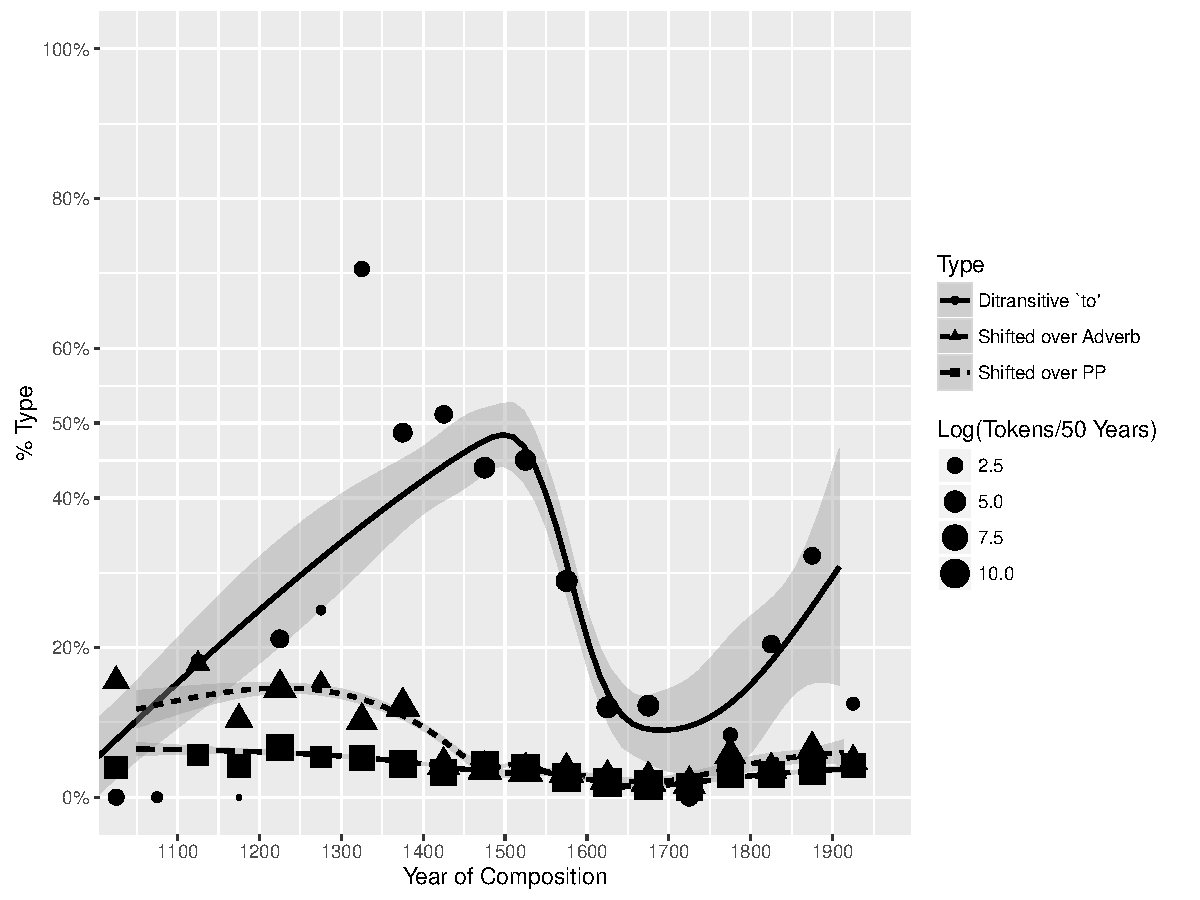
\includegraphics[width=\linewidth]{../images/shifting}
	\caption{GAM smooth over weights of `to' use in recipient--theme ditransitives and heavy NP shift over adverbs and PPs with noun phrase objects}
	\label{fig:shifting}
\end{figure}

Also, Figure \ref{fig:shifting} shows the rates of \textit{to} with recipient--theme ditransitives as well as the rates of heavy NP shift as estimated by the proportion of objects post-posed after adverbs and PPs with full noun phrase objects. Between 1450 and 1650, the rate of \textit{to} use is significantly different from the rate of heavy NP-shift ($\chi^2$ =  2365, df = 2, p < 0.001). The significant difference in rates between `to' in recipient--theme ditransitives and other post-posing operations in this time period indicates that these constructions are almost certainly \textbf{not} derived via post-posing the theme from a theme--recipient construction.

In other words, up until about 1400, \textit{to} was being used to mark recipients in all syntactic positions. In chapter \ref{ch:diachron}, I show how quantitative tools from the study of diachronic syntax are able to tease apart the initial spread of \textit{to} from the subsequent development of the allomorphy grammar. The details of the statistics can be found there, but the conclusion is that there is evidence that \textit{to} initially spread through all environments at the same rate and that a subsequent change affected the recipient--theme orders (the development of the dative shift grammar).

\section{Syntax of Recipients}\label{sec:synrecp}
The previous sections argued that recipients and goals occur in distinct syntactic constructions and that the difference between dative case and prepositions is a purely surface morphological alternation. In this section, I propose a analysis for the syntactic positions for goals and recipients. As hinted at above, I follow the rest of the literature (e.g., \citet{Jackendoff.1990,Harley.2002,Hallman.2015}) in analysing goals as being introduced in a prepositional object construction (i.e., as the object of V). For the recipient, I follow \cite{McGinnis.1998,Bruening.2010,Bruening.2010b} in assuming that the recipient is introduced in an applicative head above the VP as discussed in the previous chapter. Theme--recipient word orders are derived by scrambling the theme into a second specifier of the applicative phrase (a view first suggested for English in \citet{Takano.1998}). In the following section, I show the following: the theme can marginally reconstruct from its scrambled position (using tests for asymmetric c-command), typological evidence that the recipient--theme order is base generated and the theme--recipient order is derived, and High German specific evidence that the derivation operation is scrambling. I then further support the transformational account for English by responding to criticisms of such accounts from the literature. Finally, I use data from Low German to support the idea of scrambling even in morphologically poor languages. 
	\subsection{Asymmetric C-command}
	Binding asymmetries provide some of the clearest evidence for the internal structure of English ditransitive clauses. \cite{Barss.1986} showed that, in the recipient--theme order, the recipient systematically asymmetrically c-commands the theme. \cite{Aoun.1989} showed that, in the theme--recipient order, the theme systematically asymmetrically c-commands the recipient.  Anaphor Binding (\ref{ex:en-anaphor}), Superiority (\ref{ex:en-superiority}) and Negative Polarity (\ref{ex:en-negpol}) all show the surface c-command possibilities, in which the leftmost element asymmetrically c-commands the rightmost element (examples adapted from \cite{Aoun.1989}).
\begin{exe}
	\ex English, Anaphor Binding:\label{ex:en-anaphor}
\begin{xlist}
\ex Recipient--theme: I showed Mary herself (in the mirror).
\ex Recipient--theme: *I showed herself Mary (in the mirror).
\ex Theme--recipient: I showed Mary to herself (in the mirror).
\ex Theme--recipient: *I showed herself to Mary (in the mirror).
\end{xlist}
\ex English, Superiority:\label{ex:en-superiority}
\begin{xlist}
\ex Recipient--theme: Who did you give which check?
\ex Recipient--theme: *Which paycheck did you give who?
\ex Theme--recipient: Which check did you give to who?
\ex Theme--recipient: *Who did you give which check to?
\end{xlist}
\ex English, Negative Polarity:\label{ex:en-negpol}
\begin{xlist}
\ex Recipient--theme: I showed no one anything.
\ex Recipient--theme: *I showed anyone nothing.
\ex Theme--recipient: I showed nothing to any one.
\ex Theme--recipient: *I showed anything to no one.
\end{xlist}
\end{exe}

However, when looking at binding tests that allow for reconstruction (quantifier binding and each...the other), the recipient binding the theme is (marginally) possible in the theme--recipient order. In the recipient--theme order, the binding relationship is completely fixed. 

\begin{exe}
	\ex English, Quantifier Binding:\label{ex:en-qb}
\begin{xlist}
\ex Recipient--theme: I gave every worker$_i$'s mother his$_i$ paycheck.
\ex Recipient--theme: * I gave his$_i$ mother every worker$_i$'s paycheck.
\ex Theme--recipient: I gave every worker$_i$'s paycheck to his$_i$ mother.
\ex Theme--recipient: ? I gave his paycheck to every worker$_i$'s mother.
\end{xlist}

\ex English, Each...the other:\label{ex:en-eachother}
\begin{xlist}
\ex Recipient--theme: I showed each man the other's friend.
\ex Recipient--theme: * I showed the other's friend each man.
\ex Theme--recipient: I showed each man to the other's friend.
\ex Theme--recipient: ? I showed the other's friend to each man.
\end{xlist}
\end{exe}

German shows a similar pattern to the English data discussed above with a bias towards surface scope, such that a quantifier needs to c-command any bound pronouns on the surface. This can be seen in the recipient--theme order, where there is no availability of reconstruction (since no movement has taken place).

\begin{exe}
	\ex High German, recipient--theme:\label{ex:hg-binding-rt}
\begin{xlist}
\ex[ ]{\gll dass Maria jedem seinen Nachbarn vorgestellt hat.\\
that Maria everyone.DAT his.ACC neighbour.ACC introduced has.\\
\trans `that Maria introduced everyone his neighbor \citep[ex. 11a]{Lee.1994}.'}
\ex[*]{\gll dass Maria seinem Nachbarn jeden vorgestellt hat.\\
	that Maria his.DAT neighbour.DAT everyone.ACC introduced had.\\
	\trans `that Maria introduced everyone to his neighbour \citep[ex. 9a]{Lee.1994}.'}
\end{xlist}
\end{exe}

In the theme--recipient order, the theme can easily scope over/bind into the recipient. However, the recipient is also able to marginally scope over/bind into the theme. The judgements here are subject to speaker variation, but there are some speakers who allow the scrambled theme to reconstruct (for example to prevent a weak crossover violation). This is consistent with the idea that the theme has moved from a position under the recipient and can (marginally) reconstruct to that position at LF.

\begin{exe}
	\ex High German, theme--recipient:\label{ex:hg-binding-tr}
\begin{xlist}
	\ex[ ]{\gll dass Maria jeden seinem Nachbarn vorgestellt hat.\\
	that Maria everyone.ACC his.DAT neighbour.DAT introduced had.\\
	\trans `that Maria introduced everyone to his neighbour \citep[ex. 10a]{Lee.1994}.'}
	\ex[\%]{\gll dass Maria seinen Nachbarn jedem vorgestellt hat.\\
	that Maria his.ACC neighbour.ACC everyone.DAT introduced had.\\
	\trans `that Maria introduced everyone his neighbour \citep[ex. 12a (note 10)]{Lee.1994}.'}
\end{xlist}
\end{exe}



	\subsection{Evidence for scrambling}
	I start this section on scrambling by presenting typological evidence in support of the notion that the recipient--theme order is basic and the theme--recipient order is derived. The basic order should be available in all languages, and indeed the recipient--theme order is available in all Germanic languages:
	\begin{exe}
\ex
\begin{xlist}
	\ex \label{ex:ice-rt}
\gll P\'{e}tur gaf konunginum amb\'{a}ttina.\\
Peter.NOM gave king.DEF.DAT maid-servant.DEF.ACC.\\
\trans `Peter gave the king the maid-servant.'
\ex Faroese:\label{ex:far-rt}
\gll Hon gav Mariu troyggiuna.\\
She gave Maria.DAT sweater.DEF.ACC.\\
\trans `She gave Maria the sweater \citep{Lundquist.2013b}.'
\ex Standard Norwegian: \label{ex:nor-rt}
\gll Jeg har gitt mannen boken.\\
I have given man.DEF book.DEF.\\
\trans `I gave the man the book \citep[ex 10]{Sprouse.1995}.'
\ex Swedish:\label{ex:sw-rt}
\gll Jag gav Johan en bok.\\
I gave John a book.\\
\trans `I gave John a book \citep{Holmberg.1995}.'
\ex Danish:\label{ex:dan-rt}
\gll Peter viste jo Marie bogen.\\
Peter showed indeed Mary book.DEF.\\
\trans `Peter indeed showed Mary the book \citep{Vikner.1989}.'
\ex High German:\label{ex:hg-rt}
\gll weil er der Unehrlichkeit keine Chance gibt.\\
as he.NOM the.DAT dishonesty no.ACC opportunity gives.\\
\trans `as he gives dishonesty no opportunity \citep[162]{Draye.1996}.'
\ex Yiddish:\label{ex:yid-rt}
\gll Zi git der snjjer dus pékl. \\
she.NOM gives the.DAT daughter-in-law the.ACC parcel.\\
\trans 'She gives her daughter-in-law the parcel \citep[ex 190a]{Birnbaum.1979}.'
\ex Dutch:\label{ex:dut-rt}
\gll Ik heb (aan) Jan een boek gegeven.\\
I have (to) Jan a book given.\\
\trans `I gave Jan a book \citep{Tiersma.1985}.'
\ex Afrikaans:\label{ex:af-rt}
\gll dat die man die vrou `n dokument gegee het.\\
that the man the woman a document given has.\\
\trans `...that the man gave a document to the woman \citep{Louw.2012}.'
\ex Frisian:\label{ex:fri-rt}
\gll se joech jar kammeraatske in skjirre.\\
she gave her girlfriend a {pair of scissors}.\\
\trans `She gave her girlfriend a pair of scissors.'
\ex Low German: \label{ex:lg-rt}
\gll ick gaw den Mann dat Brod.\\
I gave the man the bread.\\
\trans `I gave the man the bread \citep{Mussaus.1829}.'
\ex English: I gave the man the book.\label{ex:eng-rt}
\end{xlist}
\end{exe}

Most of the Germanic languages\footnote{I do not have data on the availability of theme--recipient orders in Yiddish. See below for Icelandic} also allow theme--recipient word orders (as discussed above the difference between prepositions and dative case is syntactically irrelevant).

\begin{exe}
	\ex \label{ex:preprec}
	\begin{xlist}
		\ex[\%]{Faroese\footnote{Faroese is currently undergoing a change, where dative shift is becoming a regular part of the language. The \% indicates the variation seen between people, who have adopted this change versus those who have not. For those who have not adopted this change, Faroese behaves like Icelandic, which is described below.}:\label{ex:far-tr}
		\gll Hon gav telduna til gentuna.\\
		she gave computer-the.ACC to girl-the.ACC\\
		\trans `She gave the computer to the girl.'}
		\ex Norwegian:\label{ex:nor-tr}
		\gll Vi har lånt den interessante boken du nevnte *(til) Petter.\\
		we have lent the interesting book you mentioned to Peter.\\
		\trans `We have lent the interesting book you mentioned to Peter \citep{Larson.1988}.'
		\ex Swedish:\label{ex:sw-tr}
		\ex \gll Jag gav en bok *(til) Johan.\\
		I gave a book to John.\\
		\trans `I gave a book to John \citep{Holmberg.1995}.'
		\ex Danish:\label{ex:dan-tr}
		\gll Jeg gav bogen *(til) Anna.\\
		I gave book.the to Anna.\\
		\trans `I gave the book to Anna\citep{Holmberg.1998}.'
		\ex High German:\label{ex:hg-tr}
		\gll weil er keine Chance der Unehrlichkeit gibt.\\
		as he.NOM no.ACC opportunity the.DAT dishonesty gives.\\
		\trans `as he gives no opportunity to dishonesty'
		\ex Dutch:\label{ex:dut-tr}
		\gll Ik heb een boek *(aan) Jan gegeven.\\
		I have a book *(to) Jan given.\\
		\trans `I gave a book to Jan.'
		\ex Afrikaans:\label{ex:af-tr}
		\gll Ek het `n fooitjie aan hom gegee.\\
		I have a tip to him given.\\
		\trans `I have given a tip to him \citep{Stadler.1996}.'
		\ex Frisian:\label{ex:fri-tr}
		\gll ik joech in plant oan Beppe.\\
		I gave a plant to Grandmother.\\
		\trans `I gave a plant to Grandmother \citep{Tiersma.1985}.'
		\ex Low German:\label{ex:lg-tr}
		\gll ick gaw dat Brod den Man, wobei dat Brod zeigend ist.\\
		I gave the bread the man who the bread shown is.\\
		\trans `I gave the bread to the man who was shown the bread \citep{Mussaus.1829}.'
		\ex English: I gave the book to the man.\label{ex:en-tr}
	\end{xlist}
\end{exe}

	However, Modern Icelandic does not allow theme--recipient orders except as the product of heavy NP shift \citep{Dehe.2004}.

\begin{exe}
	\ex Icelandic:\label{ex:ice-tr}
\gll ?*Hann gaf amb\'attina konunginum.\\
He.NOM gave maid-servant.DEF.ACC king.DEF.DAT. \\
\trans `He gave the king the maid-servant \citep[ex 14b]{Dehe.2004}.'
\end{exe}

The universality of the recipient--theme order and the unavailability of theme--recipient orders in some languages suggest that the recipient--theme order is basic and the theme--recipient order derived (with Modern Icelandic lacking the theme--recipient deriving transformation). \cite{Georgala.2011} provides evidence from stranded depictives, floating quantifiers and split topics that all support the notion that the recipient--theme order is basic in High German. High German also provides additional evidence that the transformation under discussion is scrambling \citep{Lenerz.1977,Abraham.1986,Webelhuth.1992,Choi.1996}.

\cite{Lenerz.1977} showed that all scrambling in High German is sensitive to information focus (i.e. the focus received by new information), but not contrastive focus. In particular, words that receive new information focus cannot be targeted by scrambling operations. \cite{Lenerz.1977} applied this heuristic to ditransitives and discovered that recipient ditransitives had the following pattern. When recipients received information focus (e.g., by being the answer to a wh-question), both recipient--theme and theme--recipient word orders were possible. This would be consistent with either of the following analyses: the two word orders are not derived via scrambling or the recipient is not the element that scrambles.

\begin{exe}
	\ex High German, Recipient Focus \citep{Choi.1996}:\label{ex:hg-rec-focus}
\gll Wem hast du das Geld gegeben?\\
whom.DAT have you.NOM the money.ACC given\\
\trans `Who did you give the money to?'
\begin{xlist}
\ex \gll Ich habe dem KASSIERER das Geld gegeben.\\
I.NOM have the cashier.DAT the money.ACC given.\\
\trans `I have given the cashier the money.'
\ex \gll Ich habe das Geld dem KASSIERER gegeben.\\
I.NOM have the money.ACC the cashier.DAT given.\\
\trans `I have given the money to the cashier.'
\end{xlist}
\end{exe}

However, when the theme receives information focus, only the recipient--theme word order is possible. Given the constraints on scrambling in High German, this indicates that the recipient--theme order is base generated and that the theme--recipient order is derived via scrambling the theme above the recipient.

\begin{exe}
	\ex High German, Theme Focus \citep{Choi.1996}:\label{ex:hg-theme-focus}
	\gll Was hast du dem Kassierer gegeben?\\
what.ACC have you.NOM the cashier.DAT given\\
\trans `What did you give to the cashier?'

\begin{xlist}
	\ex[ ]{\gll Ich habe dem Kassierer das GELD gegeben.\\
I.NOM have the cashier.DAT the money.ACC given.\\
\trans `I have given the cashier the money.'}
\ex[?*]{\gll Ich habe das GELD dem Kassierer gegeben.\\
I.NOM have the money.ACC the cashier.DAT given.\\
\trans `I have given the money to the cashier.'}

\end{xlist}
\end{exe}

In Example (\ref{ex:german-VP-top}), repeated below, I presented evidence from VP-fronting that the scrambling occurs within the verb phrase. 

	\begin{exe}
		\exr{ex:german-VP-top} High German, VP-topicalisation:
		\begin{xlist}
			\ex \gll  Dem Mann das Buch gegeben habe ich, (nicht der Frau dEN Film geschenkt).\\
			the.DAT man the.ACC book given have I, (not the.DAT woman the.ACC film sent).\\
			\trans `It was giving the man the book that I did (not sending the woman the film).'
			\ex \gll Das Buch dem Mann gegeben habe ich, (nicht dEN Film der Frau geschenkt).\\
			the.ACC book the.DAT man given have I, (not the.ACC film the.DAT woman sent).\\
			\trans `It was giving the book to the man that I did (not sending the film to the woman).\\
		\end{xlist}
	\end{exe}

Another piece of evidence is that both word orders can occur after vP-level adverbs (such as negation). In combination, these facts show that the site of the scrambling is within the verb phrase.

\begin{exe}
	\ex High German, VP-level adverbs:\label{ex:hg-VPadverb}
	\begin{xlist}
		\ex \gll Ich habe nicht dem Mann das Buch gegeben, SONDERN DER FRAU DEN FILM GESCHENKT.\\
		I have not the.DAT man the.ACC book given, but the.DAT woman the.ACC film sent.\\
		\trans `I didn't give the man the book, instead I sent the woman the film.'
		\ex \gll Ich habe nicht das Buch dem Mann gegeben, SONDERN DEN FILM DER FRAU GESCHENKT.\\
		I have not the.ACC book the.DAT man given, but the.ACC film the.DAT woman sent.\\
		\trans `I didn't give the book to the man, insead I sent the film to the woman.'
	\end{xlist}
\end{exe}

\subsection{Replies to Arguments Against Transformational Analysis of English Dative Shift}

Since \cite{Oehrle.1976}, there has been an argument that English dative shift should not receive a transformational analysis, because there are interpretive differences between the recipient--theme and theme--recipient constructions. One of the interpretive differences is the existence of a completion implicature in the recipient--theme order.

\begin{exe}
	\ex Modern English:\label{ex:en-implicature}
	\begin{xlist}
		\ex[\#]{John taught the students French, but they didn't learn French}
		\ex[ ]{John taught French to the students, but they didn't learn French}
	\end{xlist}
\end{exe}

\cite{Hovav.2008} show that this completion implicature is actually the product of individual verbs and not directly attributable to the order of the objects. For example, \textit{give} entails successful transfer no matter which order the objects are in, and \textit{offer} does not entail it in either variant (it entails successful transfer in all plausible worlds in which the offer if accepted).

\begin{exe}
	\ex English, `give', \citep[exx 36 \& 37]{Hovav.2008}:\label{ex:en-implicature-give}
	\begin{xlist}
		\ex[\#]{My aunt gave my brother some money for new skis, but he never got it}
		\ex[\#]{My aunt gave some money to my brother for new skis, but he never got it}
	\end{xlist}
	\ex English, `offer', \citep[exx 38 \& 39]{Hovav.2008}:\label{ex:en-implicature-offer}
	\begin{xlist}
		\ex Max offered the victims help, but they refused his offer.
		\ex Max offered help to the victims, but they refused his offer.
	\end{xlist}
\end{exe}

\cite{Oehrle.1976} demonstrated that there were a number of different type of recipient interpretations associated even with verbs like GIVE. He argued that one of the interpretations was only available in the recipient--theme order. This interpretation involves abstract possession. The classic example is given below:

\begin{exe}
	\ex English: Nixon gave Mahler a book.\label{ex:en-nixon-rt}
	\begin{xlist}
		\ex[ ]{Nixon gave Mahler a physical object (namely a book)}
		\ex[ ]{Nixon gave Mahler an idea (that Mahler wrote into a book)}
	\end{xlist}
	\ex English: Nixon gave a book to Mahler.\label{ex:en-nixon-tr}
	\begin{xlist}
		\ex[ ]{Nixon gave Mahler a physical object (namely a book)}
		\ex[*]{Nixon gave Mahler an idea (that Mahler wrote into a book)}
	\end{xlist}
\end{exe}

These abstract interpretations inevitably involve coercing the verb into a verb of creation, since the abstract entity always comes into being by the act of giving. \cite{Frey.2001} shows that in German indefinite objects under verbs of creation have to remain in base position (i.e. they must occur to the right of manner adverbs).

\begin{exe}
	\ex High German \citep[ex 31]{Frey.2001}:\label{ex:hg-creation}
	\begin{xlist}
		\ex[ ]{\gll dass Hans geschickt eine Flöte schnitzte\\
		that John skillfully a.ACC flute carved\\
	\trans `that John skillfully carved a flute.'}
	\ex[*]{\gll dass Hans eine Flöte geschickt schnitzte\\
		that John a.ACC flute skillfully carved\\
	\trans `that John skillfully carve a flute.'}
	\end{xlist}
\end{exe}

The fact that the objects cannot scramble in German, in combination with the German predilection for surface interpretation \citep{Beck.1996}, supports the conclusion that at LF these objects need to be in their base position. That the object of verbs of creation must be interpreted in their base position explains why \textit{to} variants are generally prohibited when verbs of transfer are coerced into a creation interpretation (when the theme comes into being as part of the transfer), which \cite{Bruening.2010b} used as an argument against a transformational account of dative shift in English.

\begin{exe}
	\ex English \citep[ex. 2]{Bruening.2010b}:\label{ex:en-creation}
	\begin{xlist}
	\ex[ ]{The lighting here gives me a headache}
	\ex[*]{The lighting here gives a headache to me}
	\end{xlist}
\end{exe}

The same interpretive pressure exists in cases of idioms. Under the assumption that at LF idiomatic objects need to form a constituent with the verb in order to receive an idiomatic interpretation, scrambled idiomatic objects would need to obligatorily reconstruct promoting the recipient--theme order. Under the assumption that reconstruction is costly, there must be some countervailing pressure that would motivate the scrambling (see \citep{Bruening.2010,Bruening.2010b,Bruening.2014} for a discussion of possible motivating pressures).

\begin{exe}
	\ex English \citep[ex 3]{Bruening.2010b}:\label{ex:en-idioms}
	\begin{xlist}
		\ex[ ]{The count gives me the creeps}
		\ex[*]{The count gives the creeps to me}
	\end{xlist}
\end{exe}

The scrambling analysis is also able to more easily explain some of the purpose clause facts from \citet{Hallman.2015}. Hallman suggests that the theme--recipient order is derived via internal passivisation from the recipient--theme order (see \citet{Larson.1988}). However, he notes that this gets the standard word order between the recipient and purpose clause wrong (\ref{ex:recipient--purpose}), since the recipient would be a right adjoined adjunct in a higher phrase than the purpose clause. He is thus forced to argue that the purpose clause obligatorily scrambles above the recipient adjunct (see (\ref{ex:hallman-tree})).

\begin{exe}
	\ex \label{ex:recipient--purpose} English \citep[ex 25]{Hallman.2015}:\label{ex:en-purpose-order}
	\begin{xlist}
		\ex[*]{Mary gave a puppy to play with to John}
		\ex[ ]{Mary gave a puppy to John to play with}
	\end{xlist}
\end{exe}

In (\ref{ex:comparison-trees}), I show trees of both the scrambling analysis (following the scrambling structure provided in \cite{McGinnis.1998}) pursued here and Hallman's analysis. In both cases, the recipient scopes over the purpose clause (unlike with goals, where the goal PP scopes under the purpose clause). Under the scrambling analysis, the word order falls out without any alterations, since the recipient is still in the left attached specifier of the applicative phrase.

\begin{exe}
\ex \label{ex:comparison-trees}
\begin{xlist}
\ex Scrambling Analysis: \\
\xymatrix@=2pt{
 & vP\ar@{-}[dl]\ar@{-}[dr]\\
DP\ar@{-}[d] & & \bar{v}\ar@{-}[dl]\ar@{-}[dr]\\
\text{Mary} & \text{v} & & ApplP\ar@{-}[dl]\ar@{-}[dr]\\
 & & DP\ar@{-}[d] & & \bar{Appl}\ar@{-}[dl]\ar@{-}[dr]\\
 & & \text{the book$_{i}$}\ar@{<-}@(dl,dl)[ddrrr] & DP\ar@{-}[d] & & \bar{Appl}\ar@{-}[dl]\ar@{-}[dr]\\
 & & & \text{to John} & Appl & & VP\ar@{-}[dl]\ar@{-}[dr]\\
 & & & & & DP_{i} & & \bar{V}\ar@{-}[dl]\ar@{-}[dr]\\
 & & & & & & V\ar@{-}[d] & & CP\\
 & & & & & & \text{give}& & \text{Op$_{k}$ PRO$_{i}$ to play with t$_{k}$}}
 \ex\label{ex:hallman-tree} Hallman's Analysis: \\
 \xymatrix@=2pt{&vP_{1}\ar@{-}[dl]\ar@{-}[dr]\\
DP\ar@{-}[d] && \bar{v_{1}}\ar@{-}[dl]\ar@{-}[dr]\\
\text{Mary}&v_{1}\ar@{-}[d]&&vP_{2}\ar@{-}[dl]\ar@{-}[dr]\\
&CAUSE&\Delta&&\bar{v_{2}}\ar@{-}[dl]\ar@{-}[dr]\\
&&&\bar{v_{2}}\ar@{-}[dl]\ar@{-}[dr]&&PP\ar@{-}[d]\\
&&v_{2}&&VP\ar@{-}[dl]\ar@{-}[dr]&\text{to John}\\
&&&DP\ar@{-}[d]&&\bar{V}\ar@{-}[dl]\ar@{-}[dr]\\
&&&\text{a picture}&V\ar@{-}[d]&&CP\ar@{-}[d]\\
&&&&\text{HAVE}&&\text{Op$_{k}$ PRO$_{i}$ to play with t$_{k}$}\\}
\\
\end{xlist}
\end{exe}%13 - Tree with V' attached purpose clause

A potential problem for the scrambling analysis in English is the existence of verbs that only occur in the theme--recipient order (verbs that only occur in the recipient--theme order can be explained as lacking the scrambling operation). These verbs (e.g., DONATE) form an ill defined class that shows a great deal of inter-speaker variation \citep{Levin.1993}. I propose that there is also interspeaker variation in the orgin of the unacceptability judgements for these verbs. For some speakers, it is plausible that these verbs are analysed as introducing goals instead of recipients. In this case, the `to'-marked elements are the complement of the main verb and thus the theme--recipient order arises by default. The availabilty of goal thematic roles in Icelandic in the same situation (i.e., cases of donation) suggests that this reanalysis is plausible.

\begin{exe}
	\exr{ex:icelandic-goals} Icelandic:
	\gll \'{E}g gaf b\ae kurnar til H\'ask\'olab\'okasafnsins\\
	I.NOM gave books.the.ACC to University.Library.the.GEN\\
	\trans `I gave the books to the University Library'
\end{exe}

However, \cite{Hallman.2015} presents his judgements that suggest that even the object of these verbs are in the specifier of an applicative (namely that for him, their recipient objects are able to bind into purpose clauses). To the extent that these sentences are acceptable, the goal reanalysis is untenable.

\begin{exe}
	\ex English (ex. 48 from \citealt{Hallman.2015}):\label{ex:en-purpose-donate}
	\begin{xlist}
		\ex John donate money$_{j}$ to the church$_{i}$ [PRO$_{i}$ to buy candles with e$_{j}$].
		\ex Mary submitted a draft$_{j}$ to the professor$_{i}$ [PRO$_{i}$ to comment on e$_{j}$].
		\ex Mary returned the books$_{j}$ to John$_{i}$ [PRO$_{i}$ to reshelve e$_{j}$].
		\ex John revealed the plan$_{j}$ to Mary$_{i}$ [PRO$_{i}$ to consider e$_{j}$].
		\ex Mary demonstrated the technique$_{j}$ to John$_{i}$ [PRO$_{i}$ to teach e$_{j}$ to the new assistants].
	\end{xlist}
\end{exe}

However, a similar problem arises when looking at the behaviour of recipients in Romance languages (esp. since the English verbs are often characterised as being predominantly borrowed from Romance). The typical word order for recipients in Romance languages is theme--recipient and the recipient is obligatorily marked with a preposition (unless it has cliticised to the verb, where prepositional marking is prohibited).

\begin{exe}
\ex Italian \citep[sec. 4.3.1]{Proudfoot.2013}
\begin{xlist}
\ex \gll Ho dato il libro *(a) Paolo.\\
I.NOM gave the book to Paolo.\\
\trans `I gave the book to Paolo.'
\ex \gll Ho dato il libro *(a) LUI.\\
I.NOM gave the book to him.\\
\trans `I gave the book to HIM.'
\ex \gll (*A) gli ho dato il libro.\\
to him.DAT I.NOM gave the book.\\
\trans `I gave him the book.'
\end{xlist}
\end{exe}%22 - French examples

If the theme--recipient order is the only one that occurs, that would seem to be a refutation of the universaility of a recipient--theme base generation order, especially since requiring scrambling seems unsatisfactory. However, while theme--recipient orders are (vastly) preferred in Romance languages, there exists evidence that they are derived via the same VP-internal scrambling operation as in Germanic languages. In particular, Italian shows the same sensitivity to informaiton focus described for German, suggesting that just as in German, the theme--recipient order is derived from the recipient--theme order via scrambling.

\begin{exe}
\ex Italian \citep[ex 26]{Belletti.1995}:
\gll Che cosa hai restituto a Maria?\\
what did you.NOM {give back} to Maria?\\
\trans `What did you give back to Maria'
\begin{xlist}
\ex[ ]{\gll Ho restituto a Maria le chiavi.\\
I.NOM {give back} to Maria the keys\\
\trans `I gave back the keys to Maria'}
\ex[*]{\gll Ho restituto le chiavi a Maria.\\
I.NOM {give back} the keys to Maria\\
\trans `I gave back the keys to Maria'}
\end{xlist} 
\end{exe}%23 - Italian A-scrambling

Even though the Romance theme--recipient order is derived from VP-internal scrambling, it is necessary to explain why the operation is as restricted as it is in Romance, given that it applies much more freely in Germanic languages. At this point, it becomes useful to return to the distinction between grammar and performance discussed in Chapter 1. A grammar generates the possible utterances of the language (i.e., it creates a possibility space). However, not all grammatical possibilities are equally natural (e.g., ``the button machine with letters'' is a perfectly grammatical way of referring to a ``keyboard'', but is not the way any native speaker of English would avail themselves of). Speakers of a language conform as a community on determining how the possibilities of their grammar will be deployed in order to satisfy various demands (including information structure, prosodic naturalness, social signalling, among others). The difference between Germanic and Romance can be attributed to the way in which the possibilities generated by the scrambling grammar are deployed in actual language use.

As discussed in Chapter \ref{ch:introduction}, unacceptability can, but need not, be derived from ungrammaticality. Corpus studies of dative shift \citep{Collins.1995,Bresnan.2007,Bresnan.2009} have shown that even when all other factors are kept constant (e.g., length of objects, information status of objects, etc.), there is a great deal of between verb variation in the probability of the recipient--theme and theme--recipient word orders. \cite{Bresnan.2010} use a series of gradient acceptability judgement tasks to show that degree of acceptability of a particular word order is strongly predicted by its corpus frequency (i.e., the more likely a particular sentence is to occur in the recipient--theme order in a corpus, the more acceptable participants tended to rate it). This suggests that one source of unacceptability is an extra--grammatical dispreference for the use of certain grammatical constructions (i.e., just because a grammar generates a sentence does not mean that any native speaker of the language would use that sentence or that it will sound natural). 

By associating the DONATE class's theme-recipient preference to the independently necessary verb specific patterns of use, the grammar of recipient ditransitives can be kept simple and universal. The verb specific nature, also, explains why there is so much inter-speaker variation as to which verbs belong in the DONATE class. Each speaker needs to estimate the probability of scrambling and not-scrambling for each verb; some speakers assign such a strong lexical probability to scrambling that no other factors can override it, while other speakers assign a weaker lexical probability to the same verb moving it out of the class. The tendency for verbs of similar types to pattern together (see \citealt{Levin.1993}) can be explained by the need for speakers to often estimate lexical probability from extremely small number of attestations of a particular lexical item in their input. In those situations, a sensible strategy is to group a number of phonologically/semantically related verbs together and estimate the lexical probability of each individual verb on the basis of the group corpus.

Some evidence that DONATE does not categorically prohibit recipient--theme orders, but simply strongly disprefers them, comes from cases in which all of the other contextual factors conspire to support the recipient--theme order. This situation arises in cases of organ donation, where the recipient of the donation is animate and can be realised pronominally. In this case, (\ref{ex:kidney}) are generally judged more acceptable than (\ref{ex:donate-inanim}). Indeed, a Google search for ``donated him a kidney'' had 71 hits, suggesting that a number of English speakers find the construction grammatical.

\begin{exe}
	\ex Modern English:\label{ex:en-donate}
	\begin{xlist}
		\ex[*]{John donated him a kidney.}\label{ex:kidney}
		\ex[?]{John donated the library books.}\label{ex:donate-inanim}
	\end{xlist}
\end{exe}

\subsection{Scrambling and Overt Marking}

While scrambling has been considered a standard operation in morphologically rich languages, it has been considered rare (or impossible) in languages without overt case marking (see for example \citet{Weerman.1997}). However, Low German provides an example of a language that lacks case marking, but maintains scrambling syntax. For example, \cite{Fleischer.2006} states: ``In Low German, this construction [prepositional dative marking] could eventually be viewed as compensatory to the loss of a distinct dative case; however, from the fact that I could not find any decisive examples of this construction in Low German, I conclude that it is very rare.'' \cite{Lindow.1998} makes no mention of prepositional dative marking (including in a section discussing the uses of various prepositions. Indeed, \cite{Mussaus.1829} gives examples of theme--recipient clauses without any prepositional marking, even though the dative/accusative distinction had been lost hundreds of years before Mussäus wrote his grammar \citep{Lasch.1914,Boden.1993}.

\begin{exe}
	\exr{ex:lg-tr} Low German:
	\gll ick gaw dat Brod den Man, wobei dat Brod zeigend ist.\\
	I gave the bread the man who the bread shown is.\\
	\trans `I gave the bread to the man who was shown the bread \citep{Mussaus.1829}.'
\end{exe}

The opposite counterexample also holds, namely the only Germanic language to lack scrambling (i.e., the only language to lack theme--recipient word orders) is Icelandic, which still has rich morphological case marking.


\section{Conclusions}
In this chapter, I argued on the basis of data from active clauses that recipients are always introduced as a PP in the specifier of an applicative phrase, which means that recipient--theme word orders are always the base generated orders. Goals, on the other hand, are introduced as a direct goal PP object of the verb. The claimed universal nature of these syntactic orders supports a strong version of the Uniformity of Theta Assignment Hypothesis \citep{Baker.1988}, namely that all languages share the same base generation orders for the same theta roles.
	Typological evidence as well as language specific evidence from High German and English was brought to demonstrate that theme--recipient orders are derived from scrambling. All Germanic language have recipient--theme orders, but Icelandic lacks the theme--recipient order. High German internal evidence and data from marginal reconstruction in theme--recipient orders supports the notion that the theme is moving from a base position below the recipient to its surface position.
	The difference between dative case and prepositional marking was reduced to contextual allomorphy in the realisation of the dative P head. This morphological distinction was shown to sometimes correlate with the recipient/goal distinction, but was often independent. Evidence from Low German and Icelandic showed that the availability of scrambling is completely independent of the richness of surface morphology.

%\bibliography{diss}
